%\documentclass[11pt,a4paper]{report}


% The Beamer class comes with a number of default slide themes
% which change the colors and layouts of slides. Below this is a list
% of all the themes, uncomment each in turn to see what they look like.

%\usetheme{default}
%\usetheme{AnnArbor}
%\usetheme{Antibes}
%\usetheme{Bergen}
%\usetheme{Berkeley}
%\usetheme{Berlin}
%\usetheme{Boadilla}
%\usetheme{CambridgeUS}
%\usetheme{Copenhagen}
%\usetheme{Darmstadt}
%\usetheme{Dresden}
%\usetheme{Frankfurt}
%\usetheme{Goettingen}
%\usetheme{Hannover}
%\usetheme{Ilmenau}
%\usetheme{JuanLesPins}
%\usetheme{Luebeck}
%\usetheme{Madrid}
%\usetheme{Malmoe}
%\usetheme{Marburg}
%\usetheme{Montpellier}
%\usetheme{PaloAlto}
%\usetheme{Pittsburgh}
%\usetheme{Rochester}
%\usetheme{Singapore}
%\usetheme{Szeged}
%\usetheme{Warsaw}

\documentclass[10pt]{beamer}
\usepackage{float}
\usepackage[nodisplayskipstretch]{setspace}
\usepackage{pdfpages}
\usepackage{tikz}    
\usetheme{metropolis}
\usepackage{appendixnumberbeamer}
\usepackage[normalem]{ulem}
\usepackage{eurosym}
\usepackage{booktabs}
\usepackage[scale=2]{ccicons}
\usepackage[utf8]{inputenc}
\usepackage{soul}
\usepackage{mathabx}
\usepackage{graphicx}
\usepackage{pgfplots}
\usepgfplotslibrary{dateplot}
 \usepackage{relsize}
\usepackage{xspace}
\usepackage{caption}

\usepackage{graphicx}
\usepackage{graphicx}

\usepackage{hyperref}
\hypersetup{
    colorlinks=true,
    linkcolor=blue,
    filecolor=magenta,      
    urlcolor=blue,
}
 
\urlstyle{same}
\newcommand{\themename}{\textbf{\textsc{metropolis}}\xspace}


% As well as themes, the Beamer class has a number of color themes
% for any slide theme. Uncomment each of these in turn to see how it
% changes the colors of your current slide theme.

%\usecolortheme{albatross}
%\usecolortheme{beaver}
%\usecolortheme{beetle}
%\usecolortheme{crane}
%\usecolortheme{dolphin}
%\usecolortheme{dove}
%\usecolortheme{fly}
%\usecolortheme{lily}
%\usecolortheme{orchid}
%\usecolortheme{rose}
%\usecolortheme{seagull}
%\usecolortheme{seahorse}
%\usecolortheme{whale}
%\usecolortheme{wolverine}

%\setbeamertemplate{footline} % To remove the footer line in all slides uncomment this line
%\setbeamertemplate{footline}[page number] % To replace the footer line in all slides with a simple slide count uncomment this line

%\setbeamertemplate{navigation symbols}{} % To remove the navigation symbols from the bottom of all slides uncomment this line


\usepackage[utf8]{inputenc}
\usepackage{graphicx}

\usepackage{amsmath,amsthm,amssymb,latexsym,amsfonts}
\usepackage{tikz}
\newcommand*\circled[1]{\tikz[baseline=(char.base)]{
   \node[shape=circle,color=red,draw,inner sep=1pt] (char) {#1};}}


\setlength{\parindent}{15pt}
\usepackage{subfig}
\usepackage{hyperref}
\usepackage{graphicx} % Allows including images
\usepackage{booktabs} % Allows the use of \toprule, \midrule and \bottomrule in tables

\usepackage{bm}

\newtheorem{caution}[theorem]{¡Cuidado!}

\def\Q{\mathbb{Q}}
\def\R{\mathbb{R}}
\def\C{\mathbb{C}}
\def\N{\mathbb{N}}
\def\Z{\mathbb{Z}}
\def\S{\mathcal{S}}
\def\H{\mathcal{H}}
%\def\sde{\underset{\theta}{\times}}
\def\sde#1{\underset{#1}{\times}}

\def\G{Sea $G$ un grupo}
\def\GG{Sean\ $G, G'$\ grupos}
\def\GS{Sea\ $G$ un grupo y $S\in\S(G)$}
\def\ac{Sea $\cdot: G\times X \rightarrow X$ una acción}

\def\dcup{\sqcup}

\def\gen#1{<#1>}
\def\genn#1{<\bar{#1}>}
\def\key#1{\{#1\}}

%tetration
\def\inv#1#2{(#2,#1)}

\def\ii{\textbf{i}}
\def\jj{\textbf{j}}
\def\kk{\textbf{k}}

\def\div{por el algoritmo de división, existen $q,r$ tal que\xspace}
\def\Div{Por el algoritmo de división, existen $q,r$ tal que\xspace}
\def\m{^{-1}}

%Cambiar por un triangulito
\def\n{\Delta}

\def\p{Sea $p$ un número primo}

\def\I{[a,b]} 


\usepackage[utf8]{inputenc}
\usepackage{graphicx}
\graphicspath{ {images/} }

\usepackage[export]{adjustbox}
\usepackage{hyperref}
\usepackage{graphicx} % Allows including images
\usepackage{booktabs} % Allows the use of \toprule, \midrule and \bottomrule in tables

\usepackage{etoolbox}

\addtobeamertemplate{proof begin}{%
	\setbeamercolor{block title}{fg=black,bg=red!50!white}
	\setbeamercolor{block body}{fg=red, bg=red!30!white}
}{}


\BeforeBeginEnvironment{definition}{
	\setbeamercolor{block title}{fg=black,bg=green!20!gray}
	%\setbeamercolor{block body}{fg=black, bg=green!40!gray}
}

\AfterEndEnvironment{definition}{
	\setbeamercolor{block title}{fg=black,bg=green!20!gray}
	%\setbeamercolor{block body}{fg=black, bg=green!40!gray}
}

\BeforeBeginEnvironment{theorem}{
	\setbeamercolor{block title}{fg=black,bg=gray!40!white}
	%\setbeamercolor{block body}{fg=black, bg=green!40!gray}
}

\AfterEndEnvironment{theorem}{
	\setbeamercolor{block title}{fg=black,bg=gray!40!white}
	%\setbeamercolor{block body}{fg=black, bg=green!40!gray}
}



\title{Cuaterniones}


\begin{document}

\maketitle


\begin{frame}{Por fin, cuaterniones}

	% Bueno, les presento a los cuaterniones y continuamos el jueves.
\begin{figure}  		
  	\centering
	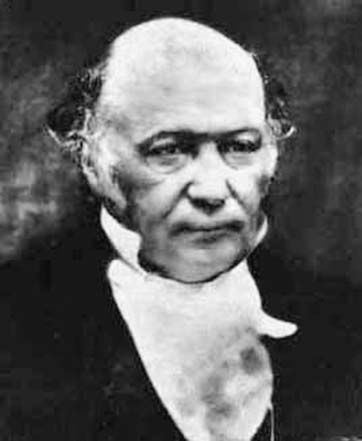
\includegraphics[scale=0.35]{images/hamilton_cara.png}
	\caption*{William Hamilton, el inventor de los horribles, \textit{horribles} cuaterniones.}
\end{figure} \pause

	% El inventor, o descubridor, si prefieren, de los cuaterniones fue un tipo que se llamaba Hamilton.
	
	% Hamilton quería generalizar el concepto de número complejo a otro objeto matemático que tuviera aplicaciones en $\R^3$
	
	% El tema es que Hamilton se imaginaba que había que agregar una sola letra imaginaria, digamos \textbf{j}. Y eso no funciona. 
Hamilton buscaba esto:
	$$a +b\cdot \textbf{i} + c \cdot \textbf{j}$$ \\
	
	($a,b,c$ son números reales) \pause
	
	...pero no funcionó.

\end{frame}

\begin{frame}

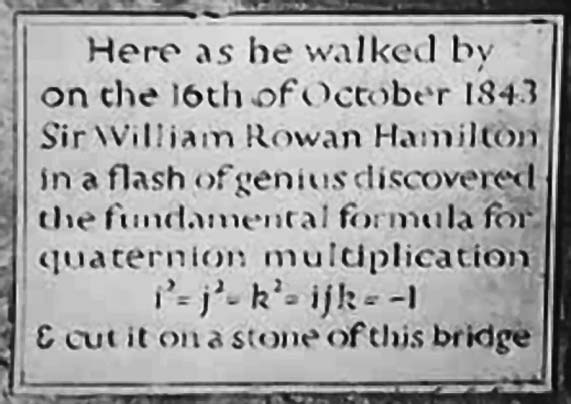
\includegraphics[scale=0.7]{images/hamilton.png}

\end{frame}

\begin{frame}{Cuaterniones}
Un cuaternión tiene esta pinta:
$$a +b\cdot \textbf{i} + c \cdot \textbf{j} + d \cdot \textbf{k}$$

	($a,b,c,d$ son números reales)  \\
	($\textbf{i},\textbf{j},\textbf{k}$ son números 'imaginarios')  \newline
	
	% Así como antes $i^2 = -1$ era la regla que usábamos para hacer cuenta, ahora estas van a ser las reglas
	

\center	Reglas:
	$$\textbf{i}^2 = \textbf{j}^2 = \textbf{k}^2 = \textbf{i}\cdot\textbf{j}\cdot\textbf{k} = -1$$ \pause 	
	% Hay algunas reglas más a tener en cuenta	
	$$\textbf{ij}=\textbf{k}\ \ \ \textbf{jk}=\textbf{i}\ \ \ \textbf{ki}=\textbf{j}$$
	$$\textbf{ji}=-\textbf{k}\ \ \ \textbf{kj}=-\textbf{i}\ \ \ \textbf{ik}=-\textbf{j}$$ \pause
	
	%O sea, i -> j -> k ->i, si multiplico dos consecutivos en orden da el otro positivo.
\end{frame}

\begin{frame}{Una representación alternativa}

Así como a un número complejo lo podíamos marcar en un plano (2 dimensiones), un cuaternión es como un vector de 4 dimensiones (no dibujable) y se puede escribir así:

$$a +b\cdot \textbf{i} + c \cdot \textbf{j} + d \cdot \textbf{k} \approx (\textbf{a},b,c,d)$$

%pero hay que tener cuidado y elegir una coordenada para que sea 'especial' ¡Fíjense que en los complejos pasaba lo mismo! La parte real era la 'especial'. Acá lo mismo.

%Se suele elegir la primera por comodidad pero tranquilamente se podría elegir otra.

\end{frame}

%TODO después de la primer charla cambiar el resumen según cómo estuvo.
\begin{frame}{Resumencito}

Los números complejos:
\begin{itemize}
	\item Se pueden marcar sumar, restar, multiplicar, dividir.
	\item Se pueden marcar en un plano.
	\item Se les puede medir la longitud y obtener el ángulo.
	\item Los de módulo $1$ representan rotaciones
	\item Para éstos, el conjugado es el inverso
	%\item Todos los complejos se pueden representar con matrices. Las matrices son el fondo funciones (transformaciones lineales)
	%\item  Algunas matrices, las que representan complejos de módulo $1$, también representan rotaciones (la función 'rotar')
\end{itemize}

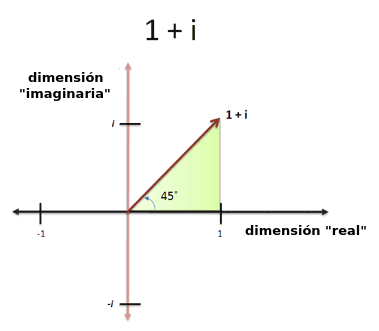
\includegraphics[scale=0.4]{images/1plusi.png}

\end{frame}

\begin{frame}{Resumencito II}
\begin{itemize}
	\item Las rotaciones en $3D$ son girar alrededor de un eje por un ángulo fijo (un pisapapas).
	\item Los cuaterniones nos van a servir para representarlas.
	\item Los cuaterniones son como los complejos pero con 2 letras más y por ende más reglas que solamente $i^2=-1$.%En particular, multiplicar no siempre conmuta. Tampoco las rotaciones en $3D$.
	%\item El producto de cuaterniones es asociativo. La suma de cuaterniones es conmutativa y asociativa.
	\item Así como los complejos se pueden ver como puntos en un plano ($2D$), los cuaterniones se pueden ver como puntos de 4 dimensiones (4 números).
\end{itemize}
\end{frame}

\begin{frame}{Tarea =)}
	¿Cómo se multiplican dos cuaterniones? ¡Usar las reglas que vimos! \bigskip
	
	$$(2+3\cdot \ii + 2 \cdot \jj - 4 \cdot \kk) \cdot (1-2\cdot \ii + 1 \cdot \jj + 4 \cdot \kk) = \text{???}$$
	
	
\end{frame}

\begin{frame}{¡Fin!}
\Huge ¿Preguntas?
\end{frame}



\begin{frame}{¡Cuidado!}
Ojo: El producto de cuaterniones en general no es conmutativo.

	% Fíjense que el producto NO es conmutativo en este caso.
	% Déjenme justificarles por qué el producto no es conmutativo de una manera intuitiva

	% Si los cuaterniones están relacionados con las rotaciones en $\R^3$ (lo vamos a ver la próxima clase) tiene sentido que si las rotaciones no son conmutativas entonces el producto de cuaterniones tampoco.
	
	% Las rotaciones en $\R^3$, ¿son conmutativas?
	
	% No. Y lo podemos ver con un cubo de rubik. Las rotaciones en $\R^3$ no son lo mismo que las de un cubo de rubik, pero sirven para generar intuición.
	
	% Si rotamos para abajo y para la izquierda no queda igual que primero para la izquierda y después para abajo.
	
	% Esto ya nos da una primer diferencia con $\R^2$
\end{frame}

\end{document}
